\subsection{Data Preparation}
The aim of this step was to get the words in the emails and use their frequency to determine whether an email is spam or ham. The HTML emails are converted to plain text to enable the building of a better vocabulary since HTML tags will not be of any use in creating the vocabulary space. Afterwards we get the word counts to vectors and output a sparse matrix. The text in the emails are then converted to their word count by stemming. Stemming allows us to create a shortened vocabulary space by getting the root of the words in the emails which in turn improves the feature space of the dataset.
\begin{figure}[H]
    \centering
    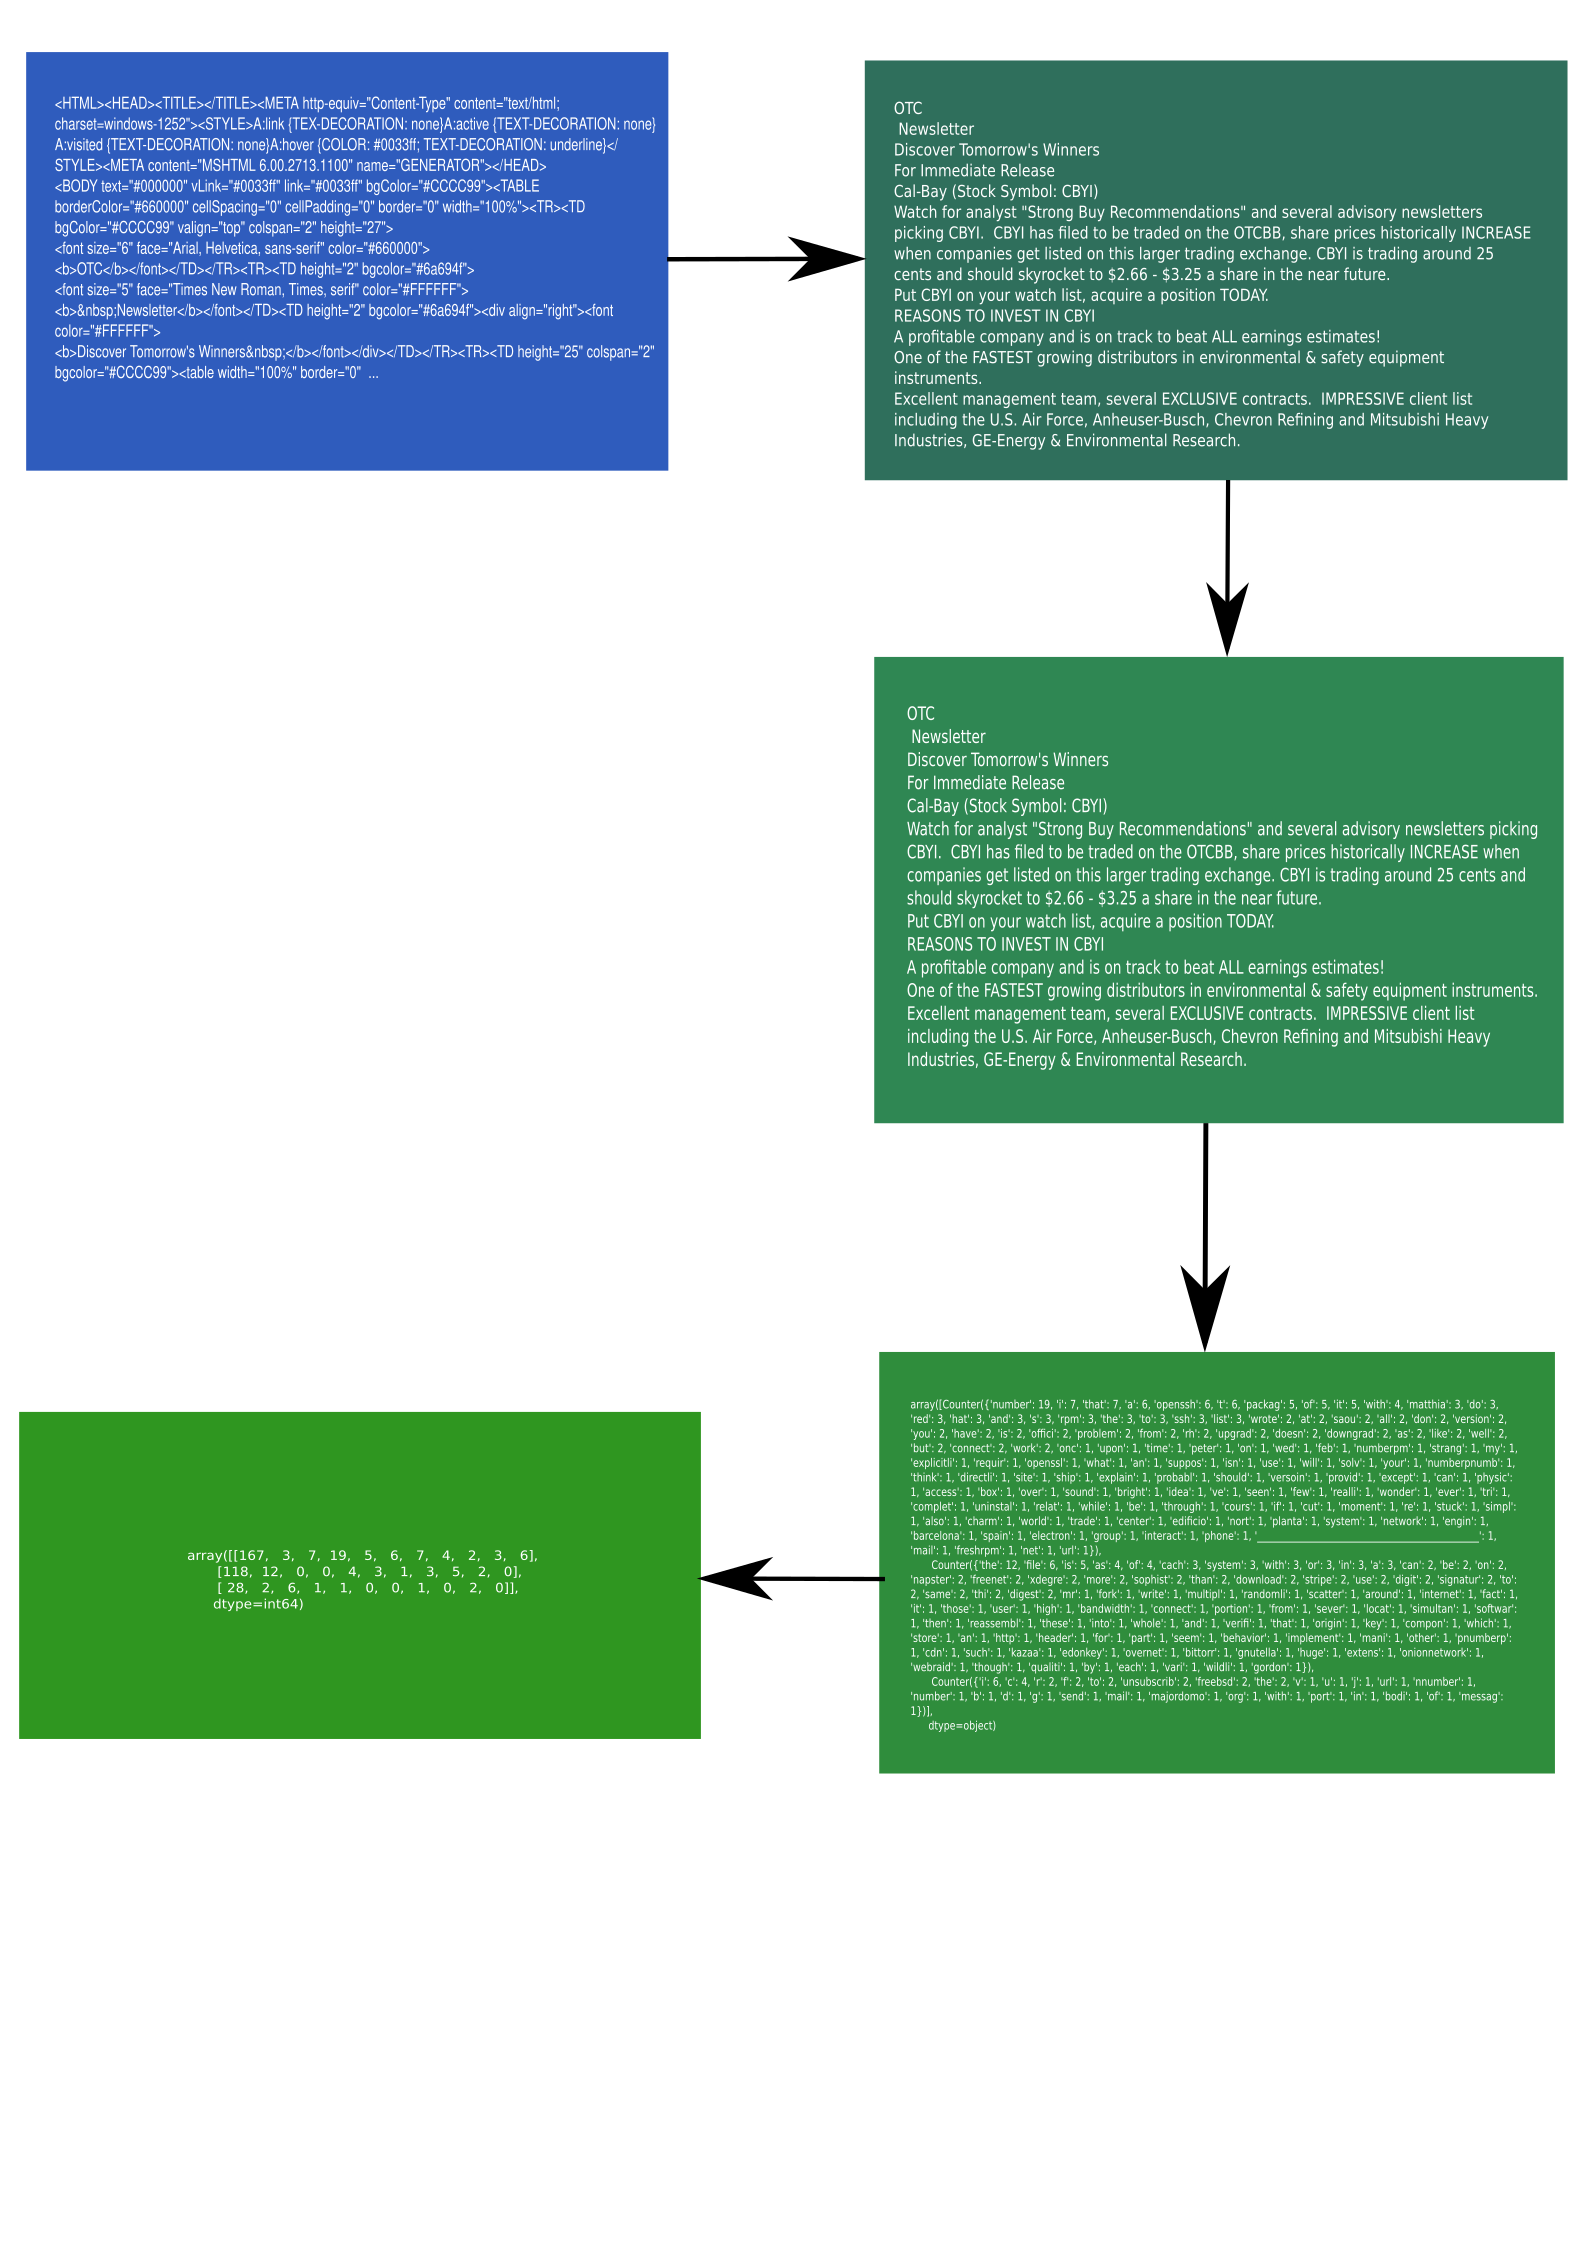
\includegraphics[width=13cm]{img/preprocessing.png}
    \caption{Data Preprocessing Steps}
    \label{fig:hybrid}
\end{figure}
